\chapter{Experiments and Results}
\label{chap:Experiments_Results}

This chapter provides the experiments and the results of this comparative study of countermeasures. As aforementioned in the last chapter, four countermeasures were selected and each one deal with one of the main cues mentioned in Section \ref{sec:SpoofingAttacksFaceRec} (liveness detection, scene characteristics and differences in image quality assessment). The countermeasures are:

\begin{itemize}
        \item Dynamic textures with $LBP-TOP$;
        \item Textures with $LBP$ \cite{ChingovskaBIOSIG2012} and \cite{maatta2011face};
        \item Motion correlation \cite{AnjosIJCB2011}.
        \item Eye blinks\footnote{https://github.com/bioidiap/antispoofing.eyeblink}.
\end{itemize}

As the Motion correlation, $LBP-TOP$ and the eye blink countermeasures need a frame sequence to work, the databases evaluated in this thesis were the Replay Attack Database (Section \ref{sec_replay}) and CASIA Face Antispoofing Database (Section \ref{sec_casia}).

The Section \ref{sec:Intra_test} presents the results applying the Intra-test protocol. Section \ref{sec:Inter_test} presents the results applying the Inter-test protocol. In the Section \ref{sec:combination} the combination of databases is explored to train each one of the presented countermeasures. In Section \ref{sec:framework} the Score Level Fusion based Framework is explored to train each countermeasure. Finally Section \ref{sec:Experiments_finalremarks} summarizes the experiments.

\section{Intra-test protocol}
\label{sec:Intra_test}

Table \ref{tb:IntraTest} shows the performance of the four countermeasures, in HTER terms, applying the Intra-test protocol.

\hspace{-17mm}\begin{table}[ht!]
\caption{$HTER(\%)$ of each countermeasure applying the intra-test ($D_1=D_2$) protocol.}
\begin{center}
  \begin{tabular}{ | c | c | c | c  c | c  c  | c  c |}
    \hline

   \multirow{2}{*}{\textbf{Countermeasure}} & \textbf{Train/Tune} & \textbf{Test} & \multicolumn{2}{c|}{\textbf{HTER(\%)}} & \multicolumn{2}{c|}{\textbf{FAR(\%)}} & \multicolumn{2}{c|}{\textbf{FRR(\%)}} \\ 
     & $D_1$ & $D_2$ & \textbf{dev} & \textbf{test} & \textbf{dev} & \textbf{test} & \textbf{dev} & \textbf{test}  \\ \hline
    
    \multirow{2}{*}{Correlation} & Replay  & Replay  &  11.66 & 11.79  & 11.66 &  & 11.66  & \\ 
               & CASIA &  CASIA  & 24.91 & 31.36 & 24.91 & & 24.91 & \\ \hline \hline

    \multirow{2}{*}{$LBPTOP_{8,8,8,1,1,1}^{u2}$}  & Replay & Replay  & 8.17 & 8.51  & 8.17& & 8.17 &\\
               & CASIA  & CASIA  & 21.77 & 22.27 & 21.77& & 21.77 &\\ \hline \hline

    \multirow{2}{*}{$LBP_{8,1}^{u2}$} & Replay  & Replay  & 14.41 &15.45 & 14.41 & & 14.41 & \\
               & CASIA  & CASIA  & 23.00  & 22.54 & 23.00 & & 23.00 &\\ \hline \hline
            
    \multirow{2}{*}{Eye blink (1 blink)} & Replay  & Replay  & 48.17 & 52.62 & 89.67 & 90.25 & 6.67 & 15.00\\
               & CASIA  & CASIA  & 48.61 &48.33 & 97.22 & 93.33 & 0.00 & 3.33 \\ \hline \hline

    \multirow{2}{*}{Eye blink (2 blink)} & Replay  & Replay  & 53.50 & 54.87 & 10.33 & 16.00 & 96.67 & 93.75\\
               & CASIA  & CASIA  & 41.67 & 44.81 & 8.33 & 6.30 & 75.00 & 83.33 \\ \hline \hline

    \multirow{2}{*}{Eye blink (3 blink)} & Replay  & Replay  & 49.17 & 49.50 & 0.00 & 0.25& 98.33 & 98.75\\
               & CASIA  & CASIA  & 47.22  & 48.89 & 2.78 & 0.00 & 91.67 & 97.78\\
    \hline
  \end{tabular}
\end{center}
\label{tb:IntraTest}
\end{table}

Analyzing the performance in the intra-test protocol ($D_1 = D_2$) it can be observed that different countermeasures have different performances using different databases. As already discussed in the Section \ref{sec_lbptop_planes}, both databases has some differences that impacts in the final performance. These differences impacted in our proposed countermeasure, based on $LBP-TOP$ (Chapter \ref{chap:Proposed_Countermeasures}), and it seems to impact in other countermeasures.

The attacks in the CASIA FASD are close-up attacks i.e. the attacker tries to fake only the face region. It is possible to see the borders of the spoofing medium and even the hands of the attacker. Additionally there are three different image qualities attacks and a bit more challenging environmental conditions. The attacks in the Replay Attack database are scenic i.e. the attacker tries to fake the face and the background at the same time in order to better fake a real access. There is no medium borders and no attackers hands. Additionally this database has two different support conditions, the fixed and the hand-held. We can consider that the CASIA FASD has only the hand-held support.

However, it is possible to observe that the $LBP-TOP$, $LBP$ and Motion correlation countermeasures have a good overall performance and, the most import, a good generalization capability. In Table \ref{tb:IntraTest} the $HTER$ in the development an in the test set are very similar indicating the assumption of generalization. The ROC curves in Figure \ref{fig:ROC_cross} corroborates this assumption. In the figure, the curves blue and red (dotted line and solid line) represents the intra-test test protocol. It can be observed that the curves are almost overlapped.

The exception here is the countermeasure based on eye blinks. In both databases de performances, in $HTER$ terms, vary from $\sim40\%$ to $\sim50\%$ independently of the number of blinks we consider, which is worse compared to the other three countermeasures.

A closer observation to the $FAR$ and $FRR$ in this countermeasure, we can conclude some things.  Considering one blink as liveness check was observed a $FAR$ of $\sim 90\%$ in both databases. Both databases has video attacks and the countermeasure capture eye blinks from there. Specially in the Replay Attack database, the hand-helded attacks introduce some noise that hits the liveness check. CASIA FASD has the warped photo attacks and these warps made by the attacker also introduce some noise deceiving the eye blink system. Also the CASIA FASD has the cut photo attacks, where the attacker uses masks of the target identity with holes in the eyes region, as can be observed in the Figure \ref{fig:blink_scene}, so in this attack the people actually blinks. 

Increasing the number of eye blinks (two and three) as a liveness check, in order to increase the robustness, the final performance is still not satisfactory. In $HTER$ terms $\sim 50\%$ in the test set in both databases. The $FAR$ now is close to $0\%$ but the $FRR$ is greater than $93\%$ in both databases. The videos in these databases are short ($\sim10s$) and it turns out that the people don't blink twice in the recording window. With these evidences of bad performances, we are no longer to support the eye blink countermeasure in this work.

\begin{figure}[!btb]
\begin{center}
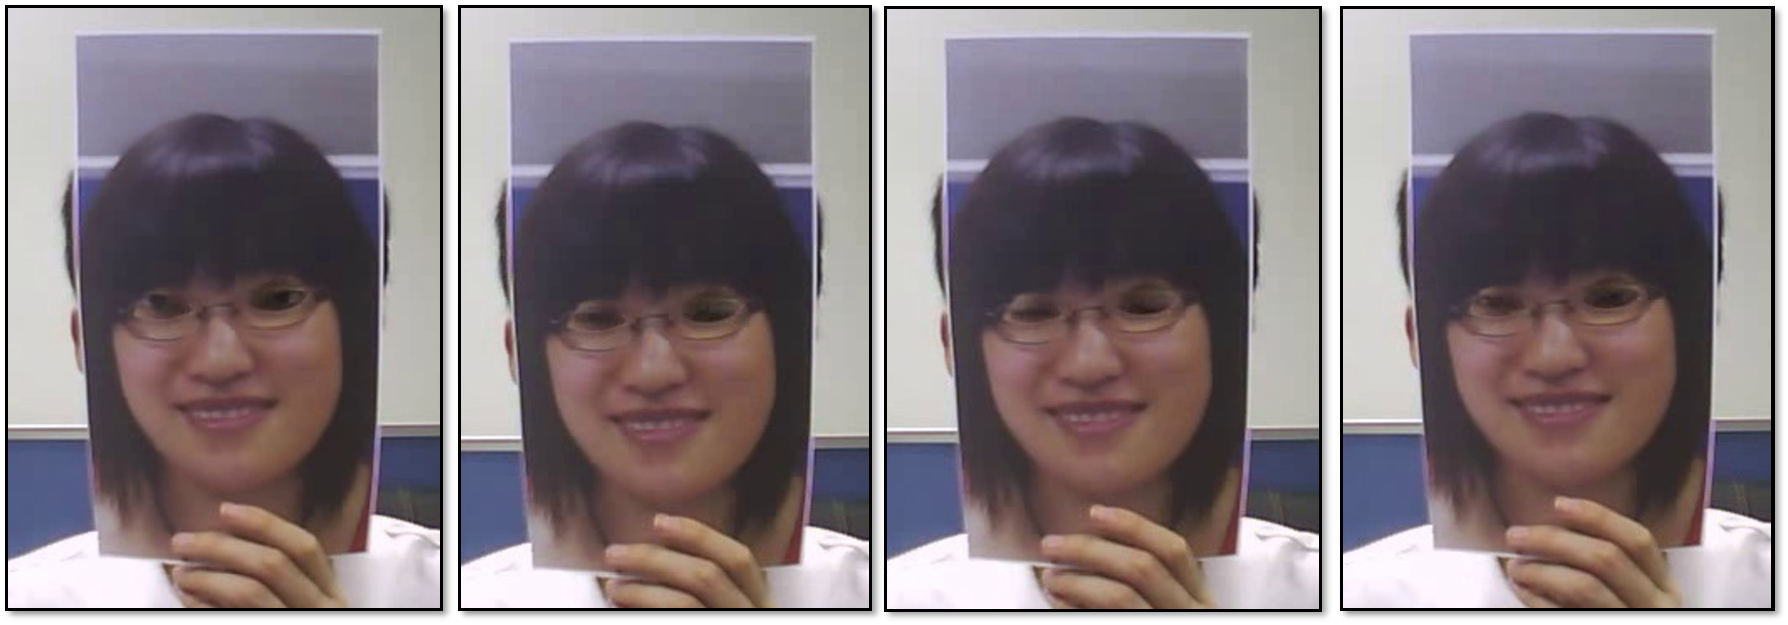
\includegraphics [width=15cm] {images/blink_scene.pdf}
\caption[Example of the cut photo attack in the CASIA-FASD]{Example of cut the photo attack in the CASIA-FASD}
\label{fig:blink_scene}
\end{center}
\end{figure}


\section{Inter-test protocol}
\label{sec:Inter_test}

Table \ref{tb:InterTest} shows the performance of the three countermeasures, in $HTER$ terms, applying the Inter-test protocol.

\hspace{-17mm}\begin{table}[ht!]
\caption{$HTER(\%)$ of each countermeasure applying the inter-test ($D_1 \neq D_2$) protocol.}
\begin{center}
  \begin{tabular}{ | c | c | c | c  c | }
    \hline

   \multirow{2}{*}{\textbf{Countermeasure}} & \textbf{Train/Tune} & \textbf{Test} & \multicolumn{2}{c|}{\textbf{HTER(\%)}} \\ 
     & $D_1$ & $D_2$ & \textbf{dev} & \textbf{test}  \\ \hline
    
    \multirow{2}{*}{Correlation} &  Replay & CASIA & 11.66 & 61.78  \\ 
               & CASIA  & Replay & 24.91 & 48.47  \\ \hline \hline

    \multirow{2}{*}{$LBPTOP_{8,8,8,1,1,1}^{u2}$}  &  Replay  & CASIA  & 8.17 & 51.05   \\
               & CASIA  & Replay & 21.77 & 61.11   \\ \hline \hline

    \multirow{2}{*}{$LBP_{8,1}^{u2}$} &  Replay  & CASIA  & 46.87  & 48.06   \\
               & CASIA  & Replay & 23.00 & 57.64  \\
            
    \hline
  \end{tabular}
\end{center}
\label{tb:InterTest}
\end{table}

Analyzing the performance in the inter-test protocol ($D_1 \neq D_2$), it can be observed that the performance results considerably degrade compared with the intra-test protocol and it becomes evident that both databases and the methods are strongly biased indicating that the countermeasures do not generalize as expected. In Table \ref{tb:InterTest} the $HTER$ in the development set and in the test set are quite different. In Figure \ref{fig:ROC_cross} the ROC curves blue and green (dashed line and solid line) representing the curves got by the development set of the database $D_1$ and by the test set of the database $D_2$ when $D_1 \neq D_2$ respectively, are quite distant from each other. The results indicate that the countermeasures and the databases can introduce some biases on the spoofing detections. The countermeasures bias are possibly related to the feature selection. The databases bias are possibly related to the differences in the databases discussed in the last Section.

Still in the biases that databases can introduce, a simple observation has to be made. In order to generate a good fake representations of a real access (without any medium borders and attackers hands), the designers of the Replay Attack database, in genenal, approximate to much the spoofing medium to the camera. It turns out that the size of the faces in the attacks are generally bigger than in the real accesses. Figure \ref{fig:database_bias} shows some examples of that observation. 

In order to see if that observation is significative in the whole database, we can run the intra-test protocol using, as a feature, only the area of the face bounding box. Table \ref{tb:TrickCounter} shows the performance of this trick countermeasure.

\begin{figure}[!btb]
\begin{center}
\includegraphics [width=16cm] {images/database_bias.pdf}
\caption[Examples of bias in the Replay Attack Database]{Examples of bias in the Replay Attack Database} 
\label{fig:database_bias}
\end{center}
\end{figure}


\begin{table}[ht!]
\caption{$HTER(\%)$ of the trick countermeasure using only the area of the face bounding box  applying the intra-test ($D_1 = D_2$) protocol.}
\begin{center}
  \begin{tabular}{ | c | c | c  c | }
    \hline

    \textbf{Tune} & \textbf{Test} & \multicolumn{2}{c|}{\textbf{HTER(\%)}} \\ 
     $D_1$ & $D_2$ & \textbf{dev} & \textbf{test}  \\ \hline
    
     Replay & Replay & 24.22 & 19.63  \\ 
     CASIA  & CASIA & 51.13 & 53.09  \\
    \hline
  \end{tabular}
\end{center}
\label{tb:TrickCounter}
\end{table}

It can be observed that for the Replay attack database the performance in the development and in the test set is far from a random behavior suggesting a bias in this database. It is not possible to observe the same shortcoming in the CASIA FASD. In next section, we stray if the countermeasures are truly biased to databases or can be tuned to overcome the database bias.

\begin{figure*}[ht]
\begin{center}
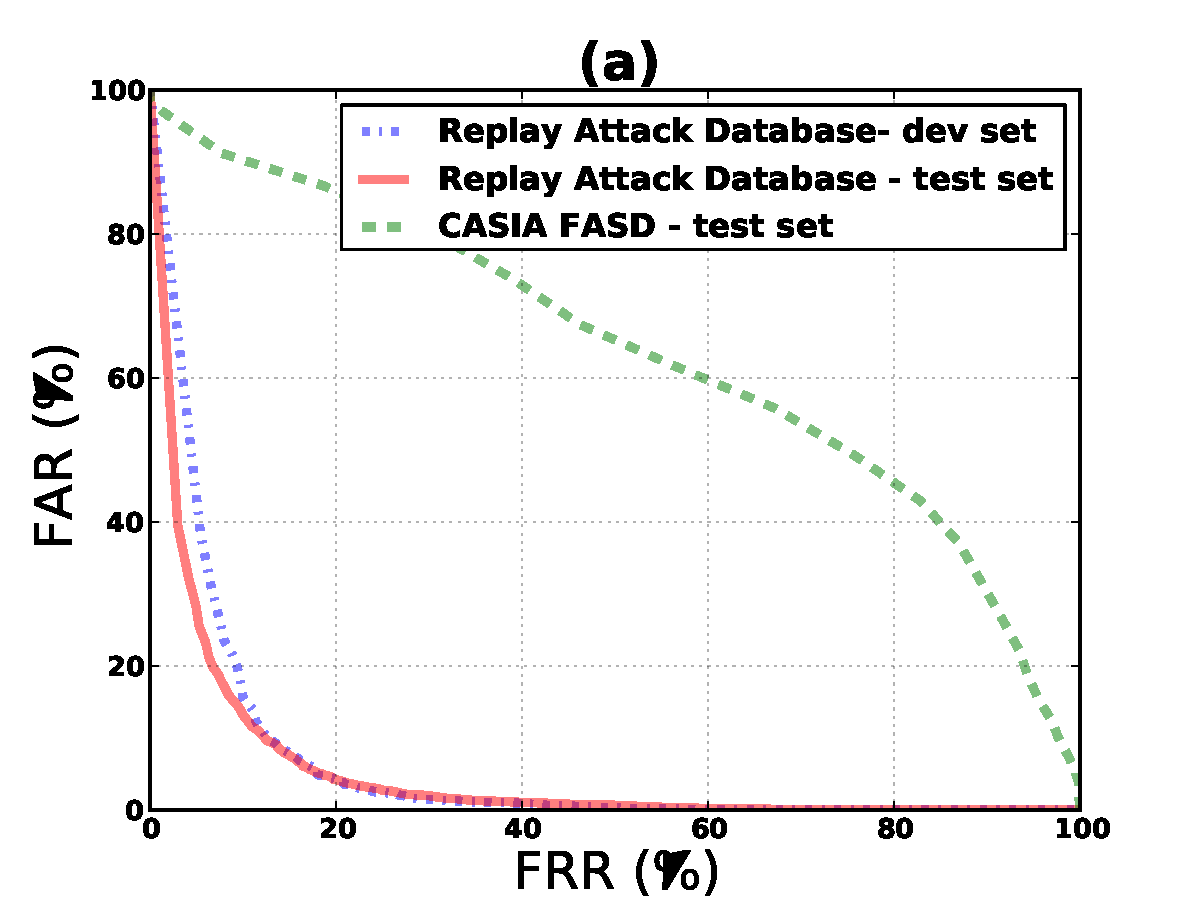
\includegraphics [width=5cm] {plots/CROSS-DATABASE/MOTION/roc_replay-machine.pdf} 
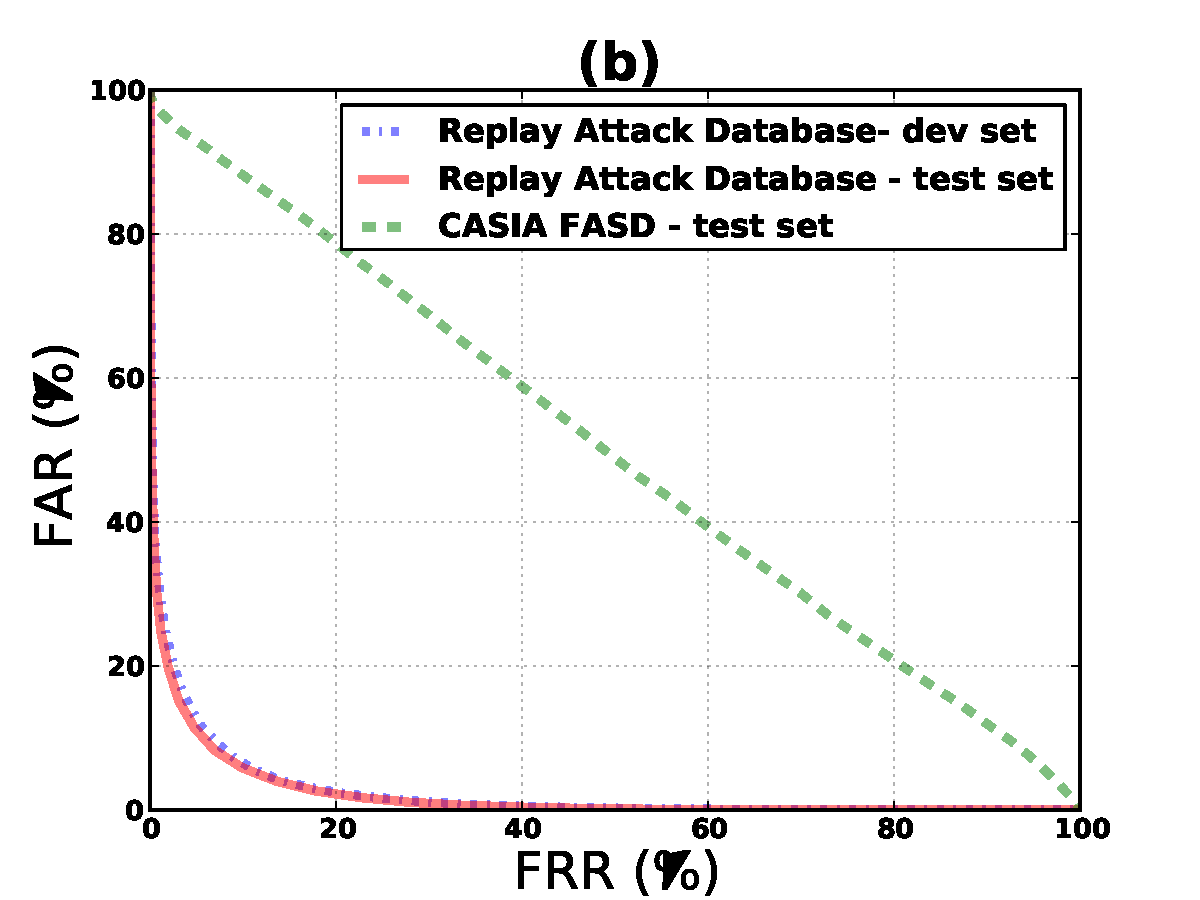
\includegraphics [width=5cm] {plots/CROSS-DATABASE/LBPTOP/roc_replay-machine.pdf}
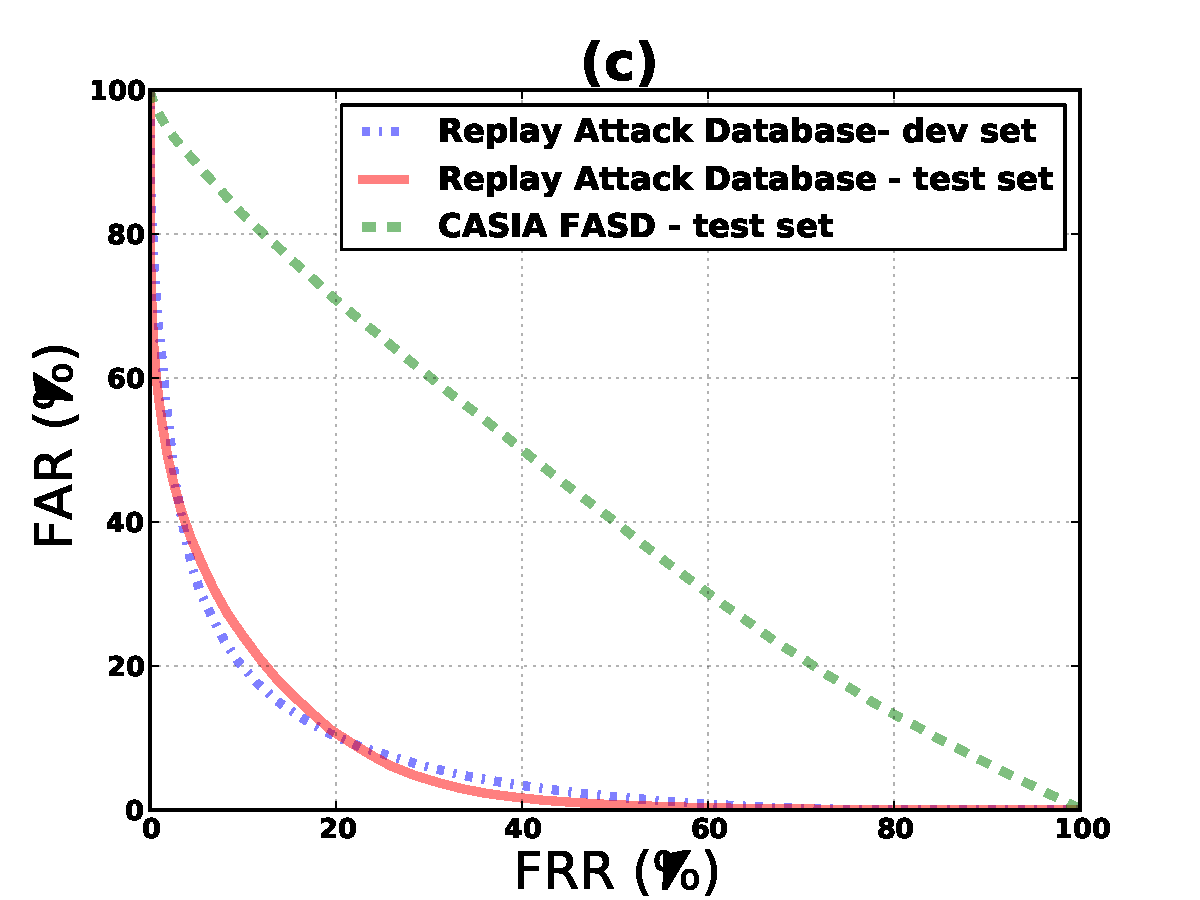
\includegraphics [width=5cm] {plots/CROSS-DATABASE/LBP/roc_replay-machine.pdf}

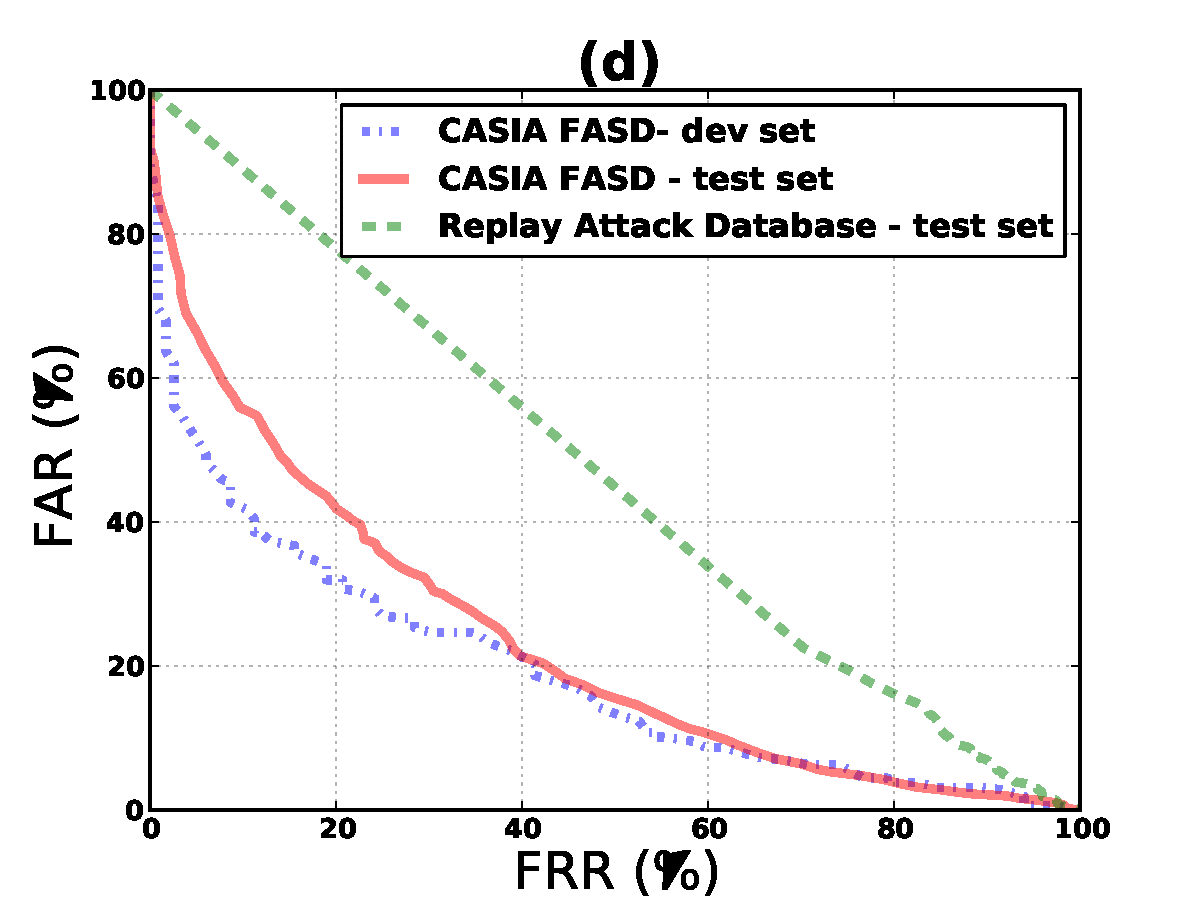
\includegraphics [width=5cm] {plots/CROSS-DATABASE/MOTION/roc_casia_fasd-machine.pdf} 
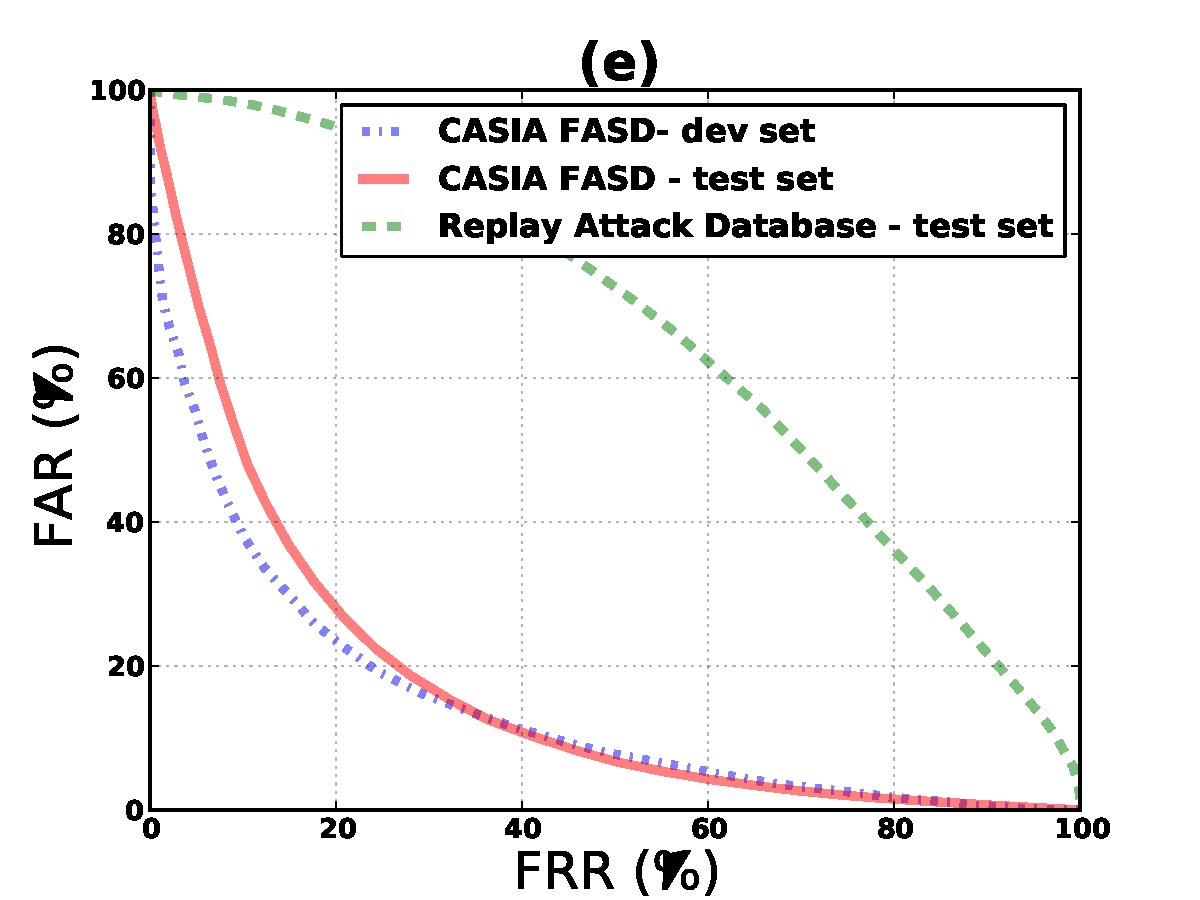
\includegraphics [width=5cm] {plots/CROSS-DATABASE/LBPTOP/roc_casia_fasd-machine.pdf}
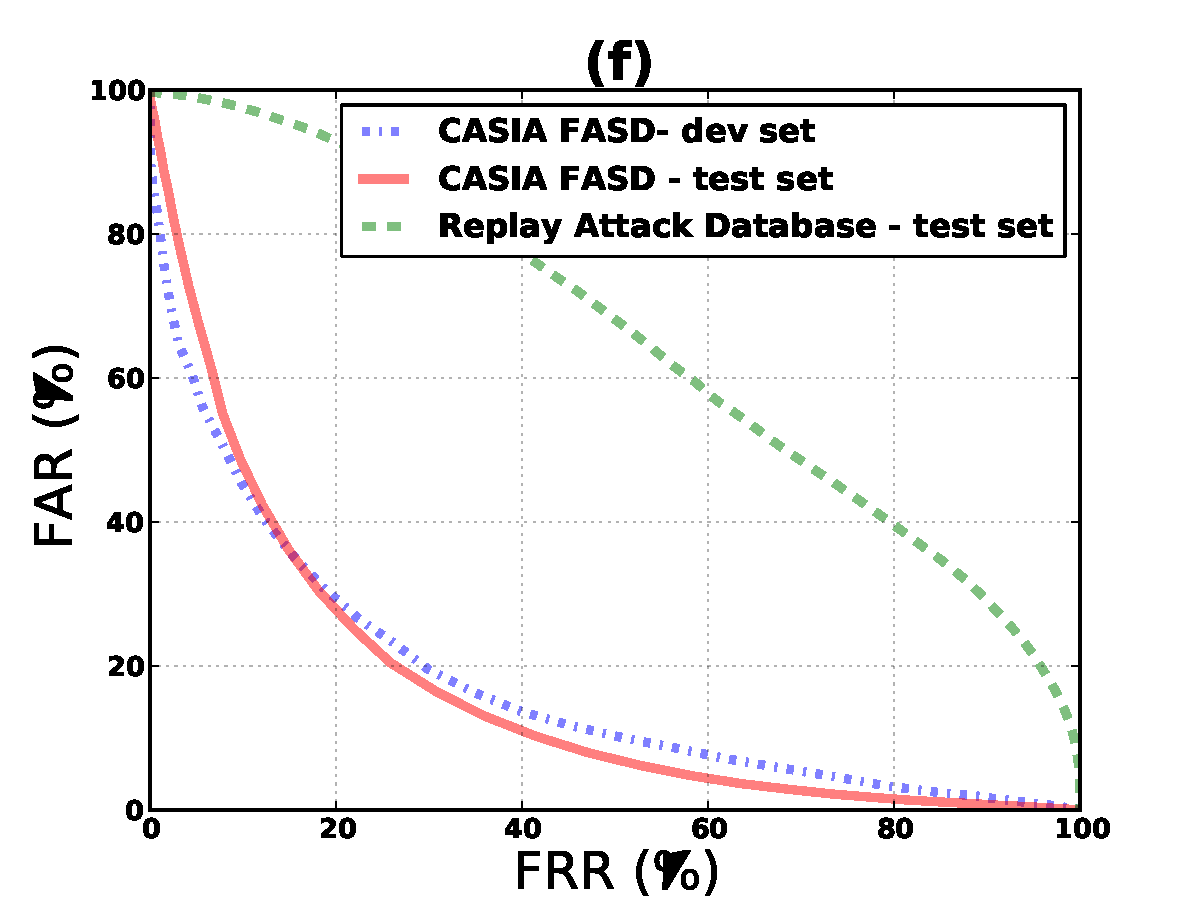
\includegraphics [width=5cm] {plots/CROSS-DATABASE/LBP/roc_casia_fasd-machine.pdf}

\caption{ROC curves of each countermeasure using the intra-test and the inter-test protocol. (a) Correlation with frame differences countermeasure trained and tuned with the Replay Attack Database (b) $LBP-TOP$ countermeasure trained and tuned with the Replay Attack Database (c) $LBP$ countermeasure trained and tuned with the Replay Attack Database (d) Correlation with frame differences countermeasure trained and tuned with the CASIA-FASD (e) $LBP-TOP$ countermeasure trained and tuned with the CASIA-FASD (f) $LBP$ countermeasure trained and tuned with the CASIA-FASD.} 
\label{fig:ROC_cross}
\end{center}
\end{figure*}


\section{Combination of Multiple Databases}
\label{sec:combination}

In the previous section we shown that, with the chosen countermeasures, was not possible to get a good performance in both databases at the same time. If we can not get that in tests with databases, what can we say about applying these in a real world scenario? If the databases introduce some bias in the countermeasures due to some particularities of them, we can train each countermeasure with a joint training set combining both databases in order to overcame these biases. This is the most intuitive approach to learn different kind of attacks. 

Table \ref{tb:TrainAllTest} shows the performance for each countermeasure trained with this strategy. %The analysis is supported with the ROC curves presented in Figure \ref{tb:TrainAllTest}.

\begin{table}[ht]
\caption{$HTER(\%)$  of each countermeasure trained with Replay Attack Database and CASIA FASD and test it with each test set of each database.}
\begin{center}
  \begin{tabular}{ | c | c | c  c |}
    \hline

   \multirow{2}{*}{\textbf{Countermeasure}} &  \multirow{2}{*}{\textbf{Test}} & \multicolumn{2}{c|}{\textbf{HTER(\%)}} \\ 
    &&\textbf{dev} & \textbf{test}  \\ \hline
    
    \multirow{2}{*}{Correlation} & Replay  &  \multirow{2}{*}{12.18} & 24.14 \\ 
               & CASIA &  & 43.30  \\ \hline \hline

    \multirow{2}{*}{$LBPTOP_{8,8,8,1,1,1}^{u2}$}  & Replay  & \multirow{2}{*}{14.29} & 10.67 \\
               &  CASIA  & & 42.04  \\ \hline \hline

    \multirow{2}{*}{$LBP_{8,1}^{u2}$}  & Replay  & \multirow{2}{*}{20.45} &19.07 \\
                & CASIA  &  & 45.92 \\
    \hline
  \end{tabular}
\end{center}
\label{tb:TrainAllTest}
\end{table}

Analyzing the performances with this strategy compared with the performance obtained with the \textbf{inter-set} protocol, can be observed a significant improvement for all three countermeasures. However, comparing with the \textbf{intra-test} protocol the performance drops drastically. It can be observed that the performance for CASIA FASD degrades more than for the Replay Attack Database suggesting a strong bias for this database. 

We can suggest that this strategy is ineffective using these countermeasures. Additionally, this strategy has one possible drawback. In face of new kinds of attacks or new databases it is necessary to train and tune all the countermeasures again. And this could be unpleasant.


%\begin{figure}[ht]
%\begin{center}
%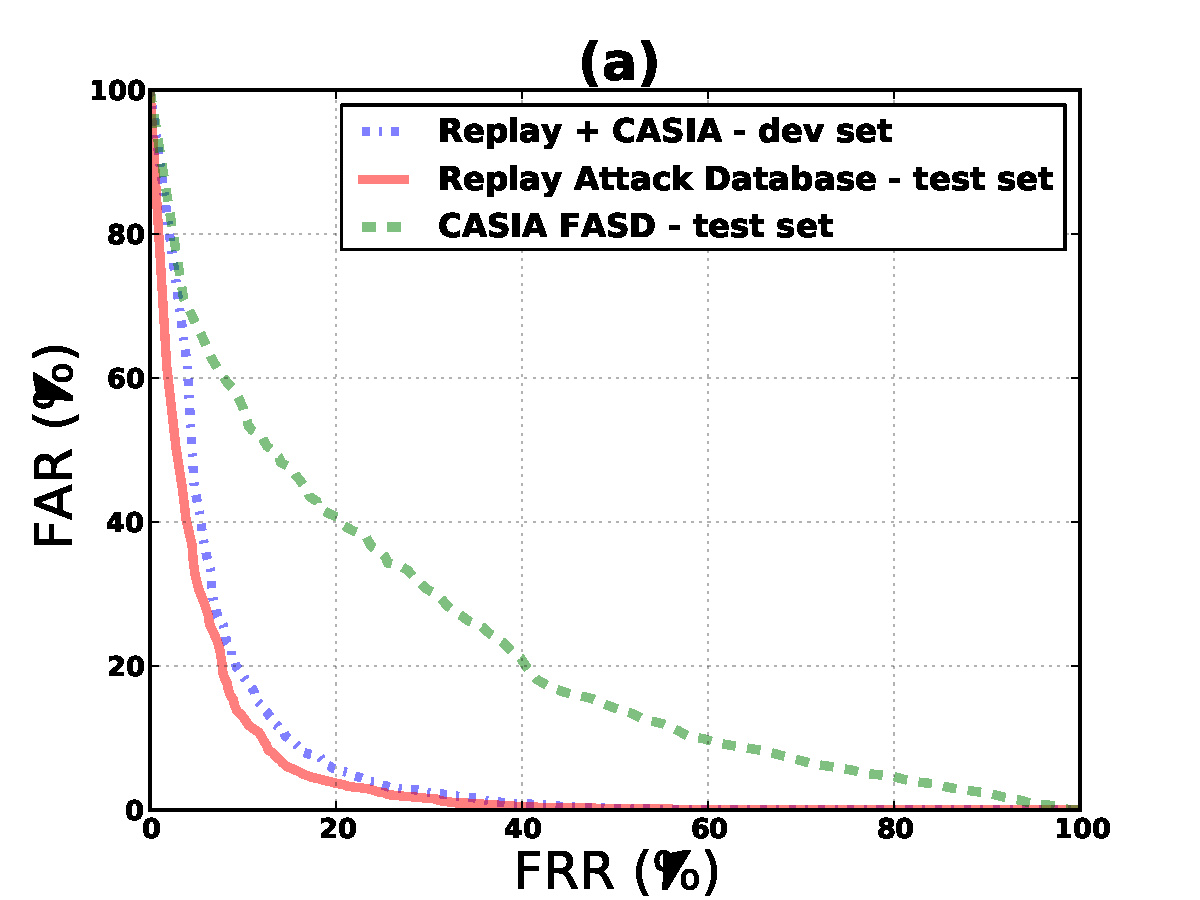
\includegraphics [width=5.5cm] {plots/ALL/MOTION.pdf} 
%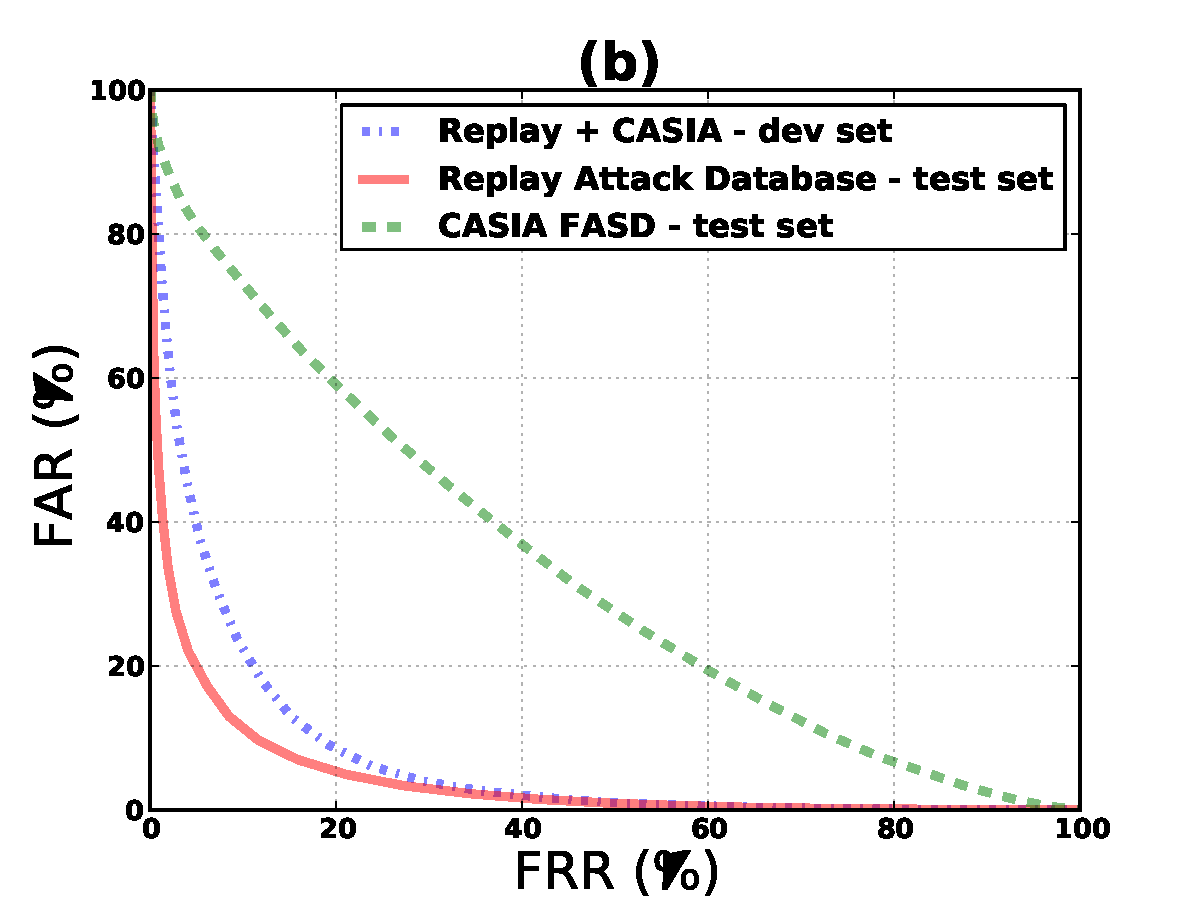
\includegraphics [width=5.5cm] {plots/ALL/LBPTOP.pdf}
%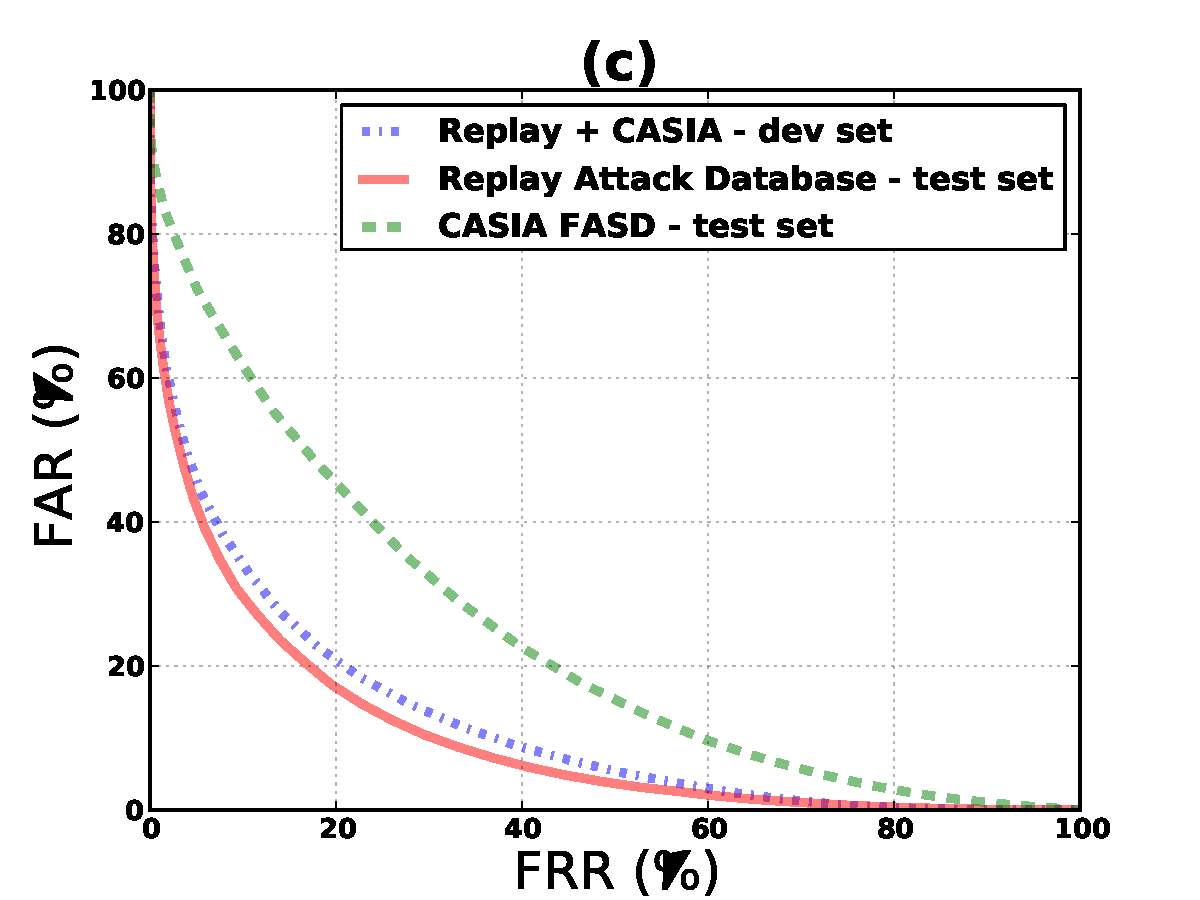
\includegraphics [width=5.5cm] {plots/ALL/LBP.pdf}
%\caption{ROC curves of each countermeasure trained with Replay Attack Database and CASIA FASD and test it with each test set of each database. (a) Correlation with frame differences (b) $LBP-TOP$ countermeasure (c) $LBP$ countermeasure} 
%\label{fig:ROC_cross}
%\end{center}
%\end{figure}


\section{Score Level Fusion based Framework}
\label{sec:framework}

In order to improve the performance results in comparison with the intra-test protocol and the inter-test protocol, and to mitigate the bias mentioned in the last section, we introduce a framework based on score level fusion. Using this framework, when a new countermeasure need to be added, it is possible to "plug it" without any extra training steps required for the other countermeasures. This strategy can be compared with an antivirus since it is possible to automatic update to new kind of attack any time such as the updates that a regular antivirus does.

To support this assumption, we first evaluate the level of independence of the countermeasures trained with different databases in order to ensure its effectiveness in a possible score fusion. Kulcheva and Whitaker \cite{kuncheva2003measures} show that the combination of statistically independent classifiers is recommended for a good performance in a score level fusion. In order to evaluate the dependence of classifiers, ten statistics were analyzed. The methodology presented in that work shows that the $Q-statistic$ is most suitable and we choose that metric to evaluate the statistic dependence of each countermeasure for the Score Level Fusion based Framework. The $Q-statistic$ for two classifiers is defined as follow:

\begin{equation}
\label{eq:Qstatistic}
Q_{R,C} = \frac{N_{11}N_{00} - N_{01}N_{10}}{N_{11}N_{00} +N_{01}N_{10}}
\end{equation}
where $R$ is the countermeasure trained with the Replay Attack Database; $C$ is the countermeasure trained with CASIA FASD; $N_{11}$ is the number of times that the countermeasure trained with the Replay Attack Database hits (i.e. correctly classifies a sample) and the countermeasure trained with the CASIA FASD also hits; $N_{10}$ is the number of times that the countermeasure trained with the Replay Attack Database hits and the countermeasure trained with the CASIA FASD misses; $N_{01}$ is the number of times that the countermeasure trained with the Replay Attack Database misses and the countermeasure trained with the CASIA FASD hits and $N_{00}$ is the number of times that the countermeasure trained with the Replay Attack Database misses and the countermeasure trained with the CASIA FASD also misses. The range of this measure goes from -1 to 1.

For statistically independent countermeasures it is expected a $Q_{R,C}$ close to 0. Results close 1 means that both countermeasures are very similar and there is no improvement in the fusion. Results close -1 indicates that both countermeasures oppose each other and a high degradation in the fusion should be expected. 

Table \ref{tb:FrameworkTest} shows the statistic dependency using the $Q-statistic$ and the performance in each database trained with the Score Level Fusion based Framework. The analysis is supported with the ROC curves presented in Figure \ref{fig:ROC_framework}.

\begin{table}[ht]
\caption{$Q-statistic$ and $HTER(\%)$ of each countermeasure trained with the Score Level Fusion based Framework and test it with each database.}
\begin{center}
  \begin{tabular}{ | c | c | c | c  c |}
    \hline

   \multirow{2}{*}{\textbf{Countermeasure}} &  \multirow{2}{*}{\textbf{Test}} & \multirow{2}{*}{\textbf{$Q_{R,C}$}} & \multicolumn{2}{c|}{\textbf{HTER(\%)}}  \\ 
     &  &  & \textbf{dev} & \textbf{test}  \\ \hline
    
    \multirow{2}{*}{Correlation} & Replay & 0.11 &  \multirow{2}{*}{13.71} & 12.39\\
               & CASIA & -0.14 &  & 32.08 \\ \hline \hline

    \multirow{2}{*}{$LBPTOP_{8,8,8,1,1,1}^{u2}$}  & Replay  & 0.24 &\multirow{2}{*}{23.16} & 26.04 \\
               &  CASIA  & -0.41 & & 38.18 \\ \hline \hline

    \multirow{2}{*}{$LBP_{8,1}^{u2}$}  & Replay  & 0.38 & \multirow{2}{*}{19.69} & 21.66  \\
                & CASIA & -0.41 &  & 47.16 \\
    \hline
  \end{tabular}
\end{center}
\label{tb:FrameworkTest}
\end{table}



\begin{figure*}[ht]
\begin{center}

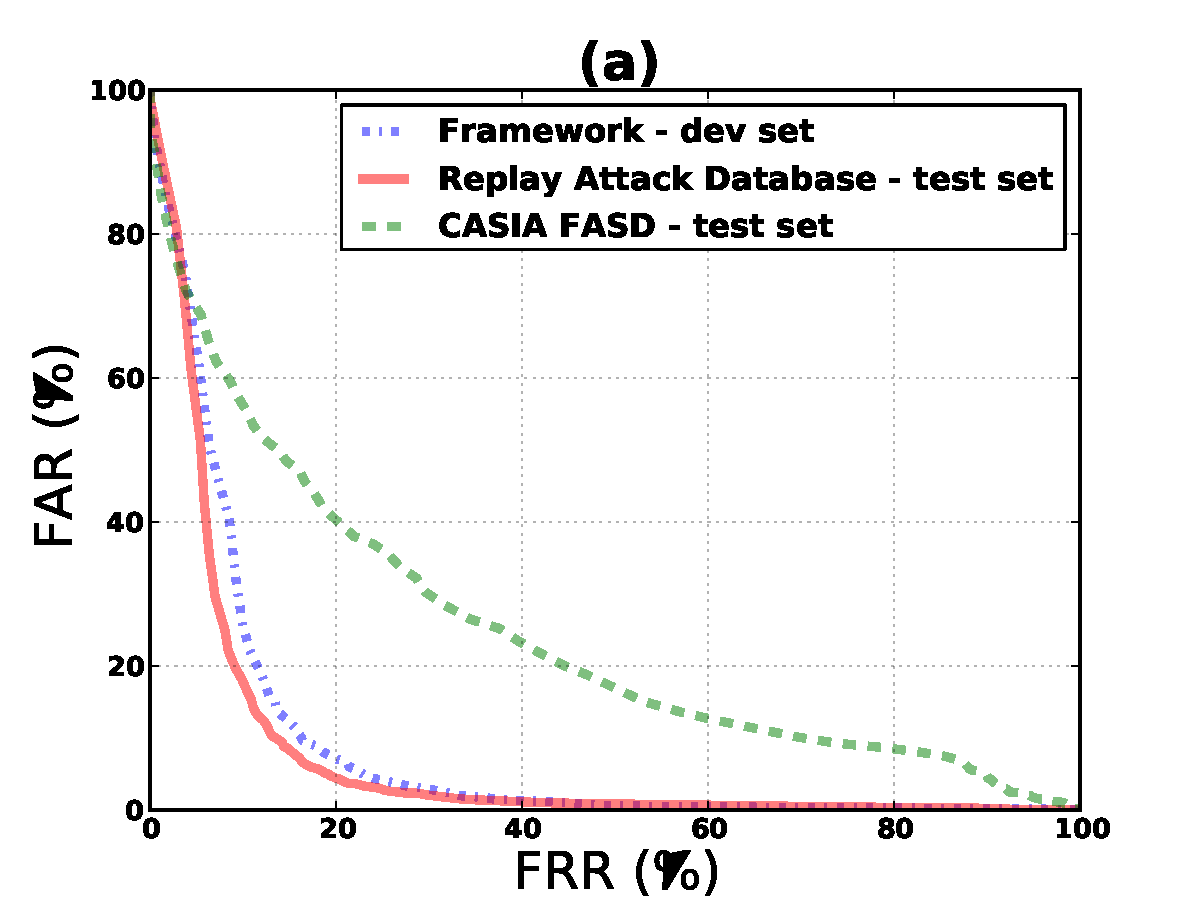
\includegraphics [width=5.5cm] {plots/FRAMEWORK/MOTION/SUM.pdf} 
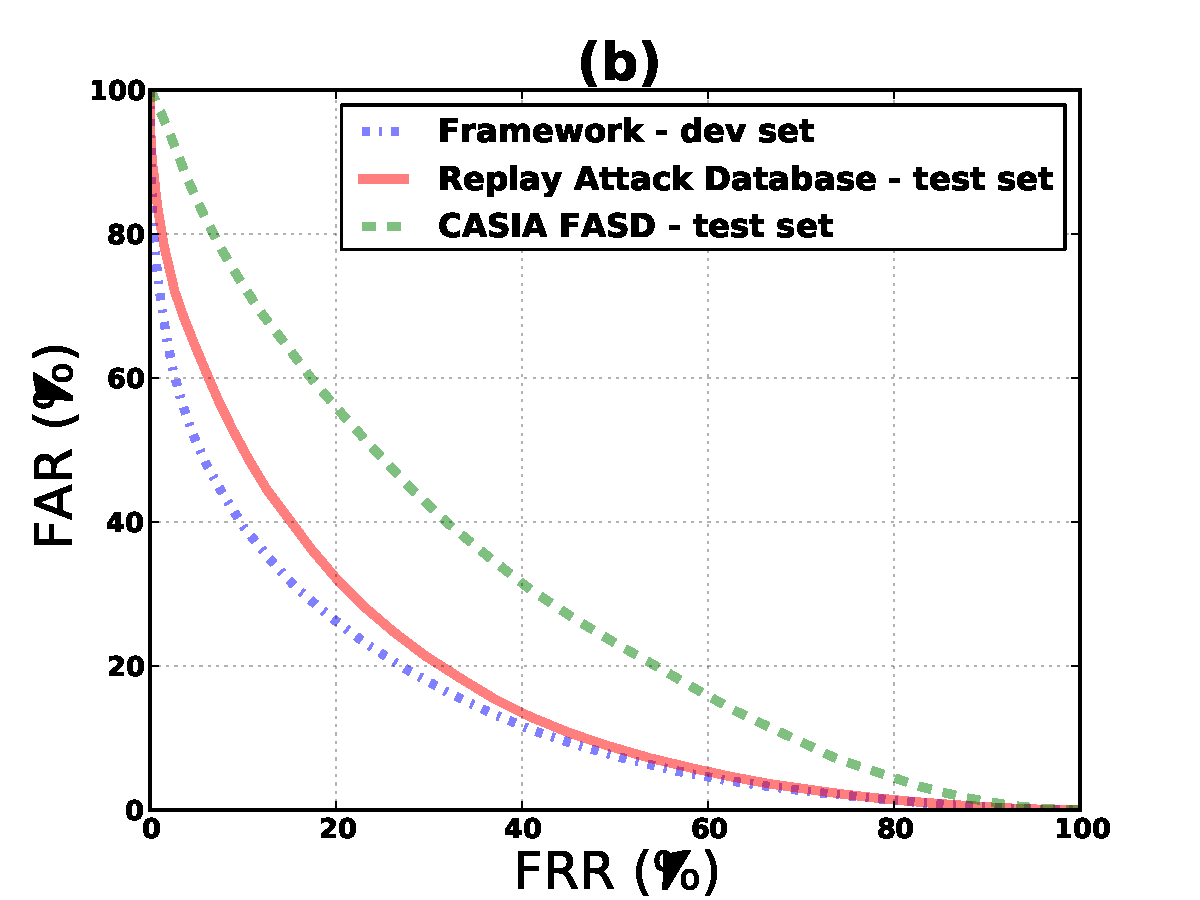
\includegraphics [width=5.5cm] {plots/FRAMEWORK/LBPTOP/SUM.pdf}
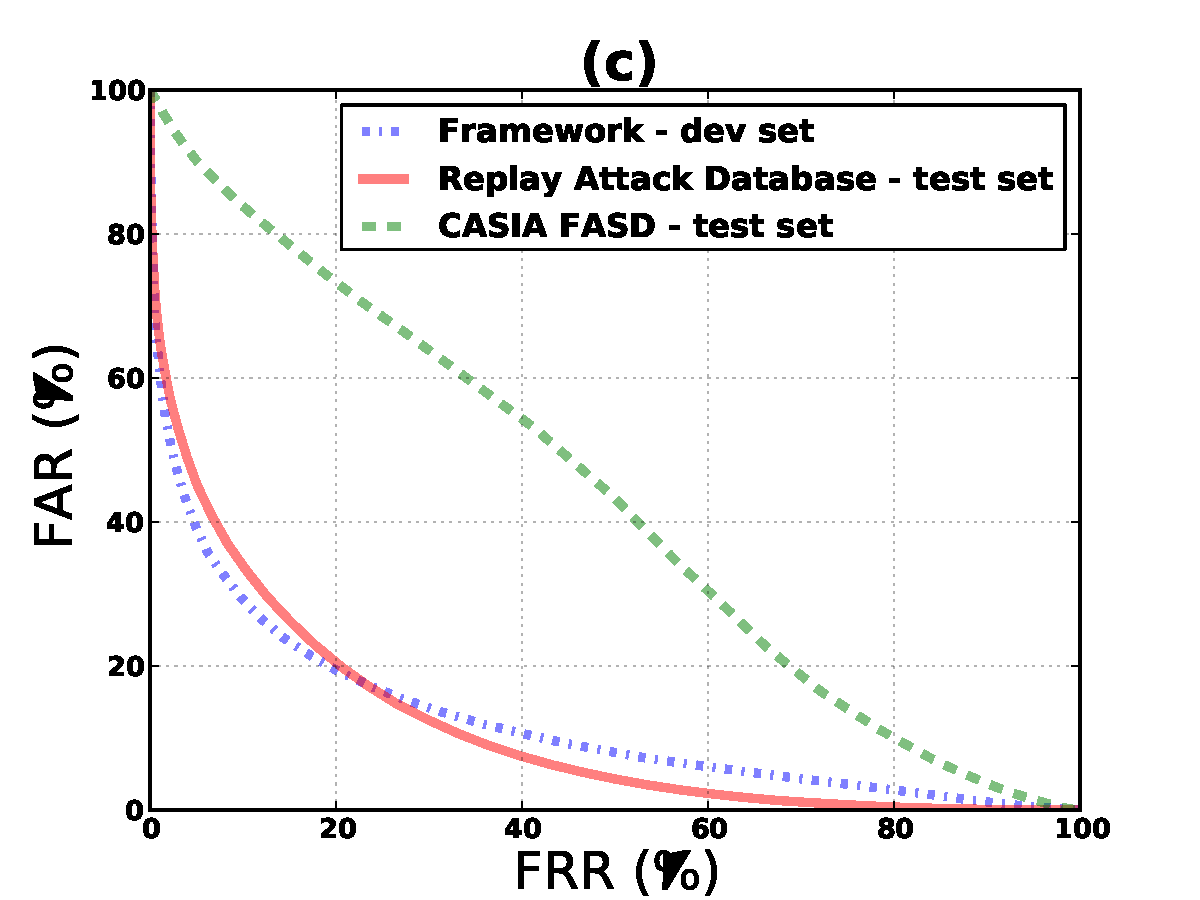
\includegraphics [width=5.5cm] {plots/FRAMEWORK/LBP/SUM.pdf}

\caption{ROC curves of each countermeasure trained with the Score Level Fusion based Framework (a) Correlation with frame differences (b) $LBP-TOP$ countermeasure (c) $LBP$ countermeasure.} 
\label{fig:ROC_framework}
\end{center}
\end{figure*}

Analyzing the $Q-statistic$ it is  possible to observe that the Correlation with Frame Differences countermeasure is the most statistically independent and suggests that a score fusion is suitable. This can be attested analysing its performance compared with the \textbf{inter-test} (see Table \ref{tb:InterTest}) and \textbf{intra-test} (see Table \ref{tb:IntraTest}) protocol results (see Table \ref{tb:FrameworkTest}). For the inter-test protocol the improvement with the Score Level Fusion based Framework was significative. Comparing with the intra-test protocol the degradation was very low and the countermeasure is able to detect spoofs in both databases with different degrees of success.

However the $Q-statistic$ for the $LBP-TOP$ and the $LBP$ countermeasures present unbalanced values for each database. Specially for the CASIA FASD $Q_{R,C}\simeq-0.4$ suggesting that each one of this two countermeasure trained with different databases oppose each other and are not suitable for the Score Level Fusion based Framework. This can be attested analysing their performances compared with the intra-test protocol results (see Table \ref{tb:IntraTest}). The degradation is still high.

%The authors that designed the $LBP$ and $LBP-TOP$ countermeasures chosen the SVM with the RBF kernel as classifier. In both settings, the final trained machines have $\sim35\%$ of the training data as support vectors, what suggest overfitting in each database. The authors that designed the Correlation with Frame Differences countermeasure chosen MLPs with only 5 neurons, which is much simpler classifier and has less chance to overfit of the training data than a SVM.

It is important to remark that the literature lacks in video face spoofing databases and is not possible to ensure the effectiveness of the Score Level Fusion based Framework in a third database. Its effectiveness in a third video face spoofing database, at this stage is only speculative. Another point to highlight is that the fusion strategy chosen for this work is quite simple. For a future extensions more complex fusion strategies need to be addressed.

\section{Final Remarks}
\label{sec:Experiments_finalremarks}

This chapter compared four countermeasures, very representative according to the state of the art of this research field, using two different test protocols. Using the only two video face antispoofing databases publicly available (Replay Attack Database and CASIA FASD) we introduced the intra-test protocol and the inter-test protocol.

The evaluation of each countermeasure using the intra-test protocol, suggests a good performance and good intra-database generalization power for three countermeasures (Textures with $LBP$, Dynamic textures with $LBP-TOP$  and Motion Correlation). The exception was the countermeasure based on eye blinks. Due to some particularities of the databases, this countermeasure was not effective in this protocol and we discarded it. Using the inter-test protocol, the countermeasures accumulates a lot of degradation suggesting a strong bias in the databases.

To overcame this bias we introduce two approaches. The first one, combination of multiple databases, combines the train set of each database to train each one of the presented countermeasures. Compared with the inter-test protocol, this strategy improved the countermeasures performance. However, it was observed a strong bias to the Replay Attack Database degrading the performance in the CASIA FASD comparing with the intra-test protocol. In the second approach, we introduced the Score Level Fusion based Framework that merges the scores of countermeasures trained with different databases. Only countermeasures that are statistically independent are suitable for an effective score fusion. Analyzing the $Q-statistic$ measure, the Correlation with Frame Differences countermeasure is the most statistically independent and it is the most suitable for the Framework. This was attested comparing the performance of this countermeasure with the performance obtained with the inter-test and intra-test protocols.  However the framework performance using the $LBP-TOP$ and $LBP$ presented unbalanced values for each database and high absolute values for the $Q-statistic$. This behavior indicated the "improperness" of fusion for these countermeasures.

